\documentclass[a4paper,12pt]{report}    %Article before

\usepackage{preamb}

\begin{document}

\lstset{style=output}
\thispagestyle{empty}
\centerline{\fontsize{60}{70}\selectfont\textbf{Embedded Real Time Systems}}
\vspace{10mm}
\vspace{40mm}
\centerline{\Huge\textbf{Assignment 2}}
\vspace{40mm}

\begin{table}[htb]
\fontsize{16}{30}\selectfont
\centering
\begin{tabular}{| p{85mm} | p{60 mm} |}
\hline
\textbf{Name:}                      &  \textbf{Students number:}     \\ \hline
Malthe Faurschou Tøttrup            &  201907882                     \\ \hline
Jakob Levisen Kvistgaard            &  201606374                     \\ \hline
\end{tabular}
\end{table}

\vspace{10mm}
\vspace{20mm}

\centerline{\large\textbf{\today}}
\centerline{\large\textbf{ }}


\tableofcontents
\pagestyle{ProjectReport}
\newpage
\lstlistoflistings
\newpage

\chapter{Assignment 1}
\section{Introduction}

The is the first assignment in Embedded Real Time Systems.
All source files can be found at: \url{https://github.com/levisen/ERTS}






\section{ModuleSingle}

The first module implemented is a single threaded method run every 2ms. 

\lstset{style=code}
\lstinputlisting[language=C++, firstnumber=6, firstline=6, lastline=18, caption=Implementation of single.h header., label=31HEADER]{../code/src/assignment1/ModuleSingle/single.h}

\lstinputlisting[language=C++, firstnumber=4, firstline=4, lastline=14, caption=Implementation of single.cpp source., label=31SOURCE]{../code/src/assignment1/ModuleSingle/single.cpp}

As we are using a \textbf{sc\_uint<4>} type, the maximum for the counter will be \( 2^4 = 16 \). Which is noticed in the output \ref{31OUT}, whenever the counter reaches 15. As the counter goes from 0-15.

\lstset{style=output}
\lstinputlisting[firstline=12, lastline=17, caption=Output result from exercise 3.1., label=31OUT]{../code/src/assignment1/ModuleSingle/out/out}






\section{ModuleDouble}

For this exercise, we define the 4 events, 2 threads, and the method to be called from both threads in \ref{32HEADER}.

\lstset{style=code}
\lstinputlisting[language=C++, firstnumber=6, firstline=6, lastline=22, caption=Implementation of double.h header., label=32HEADER]{../code/src/assignment1/ModuleDouble/double.h}

Both of the threads are essentially implemented the same way. Just with different names shown in listing \ref{32SOURCE}. The \textbf{next\_trigger()} method is called to actively trigger the next event.

\lstinputlisting[language=C++, firstnumber=12, firstline=12, lastline=26, caption=Implementation of double.cpp source., label=32SOURCE]{../code/src/assignment1/ModuleDouble/double.cpp} 

In listing \ref{32OUT} it is seen that B is acknowledged every 2 ms, until a - that has a timeout period on 3 ms - gets called. Because A has catched up to 6ms and both ack should be called. B is skipped due to the thread's method is alternating. With the result of Back's next message being delivered at 8 ms.

\lstset{style=output}
\lstinputlisting[firstline=1, lastline=6, caption=Output result from exercise 3.2., label=32OUT]{../code/src/assignment1/ModuleDouble/out/out}





\section{ProducerConsumer}

Here, we are using the \textbf{sc\_fifo<>} type to initialize two \textbf{TCPHeader*} dummy instances, that represent the physical ports. 

\lstset{style=code}
\lstinputlisting[language=C++, firstnumber=8, firstline=8, lastline=27, caption=Initialization source for Producer Consumer implementation in SystemC., label=33HEADER]{../code/src/assignment1/ProducerConsumer/top.h}

The producer thread waits randomly and then generates a new \textbf{TCPHeader} instance to write to the \textbf{sc\_port}. Essentially the \textbf{TCPHeader} could be any dummy data object, that we want to transfer. Using the \textbf{package\_number} listed in \ref{33SOURCE::PRODUCER}, we incremented the package counter to keep track of sent packages to the consumers. The magic happens with the \textbf{sc\_fifo\_in<>} type, which clarifies the use of a FIFO port in SystemC. As shown in listing \ref{33SOURCE::CONSUMER}, the message from the physical port handled by SystemC, is consumed when the \textbf{read()} function is called.

\lstinputlisting[language=C++, firstnumber=4, firstline=4, lastline=15, caption=Implementation of producer.cpp source, label=33SOURCE::PRODUCER]{../code/src/assignment1/ProducerConsumer/producer.cpp}

\lstinputlisting[language=C++, firstnumber=4, firstline=4, lastline=9, caption=Implementation of consumer.cpp source, label=33SOURCE::CONSUMER]{../code/src/assignment1/ProducerConsumer/consumer.cpp}

The results listed in listing \ref{33OUT}, show the consumer name initialized in listing \ref{32HEADER}, sequence number and at which time the messages is generated and put to the queue. For some fun at the transport layer level, where this packages is typically used, we also added a random destination port.

\lstset{style=output}
\lstinputlisting[firstline=1, lastline=6, caption=Output result from exercise 3.3., label=33OUT]{../code/src/assignment1/ProducerConsumer/out/out}





\section{MasterSlave}
A cycle accurate communication model has been implemented using the figures from the exercise. Essentially the \textbf{data},\textbf{ready} and \textbf{valid} is the most interesting to look at, as the other signal are sending dummy data in this implementation.


\lstset{style=code}
\lstinputlisting[language=C++, firstnumber=8, firstline=8, lastline=40, caption=Initialization source for Master Slave implementation in SystemC., label=34HEADER]{../code/src/assignment1/MasterSlave/top.h}

The \textbf{produce()} - shown in listing \ref{34PRODUCER} - function is implemented through a set of if/else in a while loop, invoked by the thread. For every cycle in the loop we read the data, and depending on whether the slave is ready to consume the next message, we set the \textbf{valid} signal to true and write. 

\lstinputlisting[language=C++, firstnumber=19, firstline=19, lastline=48, caption=Master implementation for Master Slave., label=34PRODUCER]{../code/src/assignment1/MasterSlave/master.h}

For the slave implementation, we read every cycle and if the \textbf{valid} signal is true, we simply save the data. For simulation purposes, we randomize the \textbf{ready} signal of the unit, to simulate some processing. Which would usually occur on such devices.

\lstinputlisting[language=C++, firstnumber=21, firstline=21, lastline=43, caption=Slave implementation for Master Slave., label=34CONSUMER]{../code/src/assignment1/MasterSlave/slave.h}

The end result listed in \ref{FIG::34} shows that whenever the \textbf{clock} signal goes high, is where the data is written to the signal port. It also indicates that both \textbf{valid} and \textbf{ready} must be high for the data to be written and acknowledged.

\begin{figure}[h]
  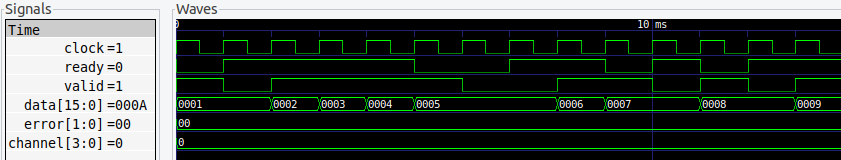
\includegraphics[width=\linewidth]{../code/src/assignment1/MasterSlave/out/out.png}
  \caption{Gtkwave output from simulation}
  \label{FIG::34}
\end{figure}






\section{InAdapter}

For the InAdapter one can implement another master node to feed data into the system. By following the 'Adapter Model' design from the exercise, we first implemented the Master. This is just a dummy producer node that increments data over time.

\lstinputlisting[language=C++, firstnumber=6, firstline=6, lastline=20, caption=Producer from master.h source file., label=35PRODUCER]{../code/src/assignment1/InAdapter/master.h}

With the implementation of the InAdapter already provided, one can continue with the slave, which is essentially the same implementation as in listing \ref{34CONSUMER}. We now use predefined SystemC logic types instead of just integer values. This is shown in listing \ref{35CONSUMER}.

\lstinputlisting[language=C++, firstnumber=18, firstline=18, lastline=42, caption=consume method from slave.h  source file., label=35CONSUMER]{../code/src/assignment1/InAdapter/slave.h}

In general, the results look somewhat similar compared to the results in the previous exercise in figure \ref{FIG::34}. We see that the results differ, whenever a signal has been sent, as after acknowledgment, the \textbf{valid} signal goes back to low. 

\begin{figure}[h]
  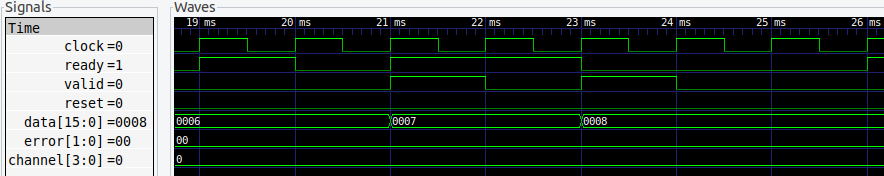
\includegraphics[width=\linewidth]{../code/src/assignment1/InAdapter/out/out.png}
  \caption{Gtkwave output from simulation}
  \label{FIG::35}
\end{figure}



\end{document}
